\documentclass{beamer}

% ako se sledeca komanda izostavi, bice upotrebljena default tema
\usetheme{Warsaw}

% Packages
\usepackage{listings}
\usepackage{amsmath,amssymb,lmodern}

% Defines section title page
\AtBeginSection[]{
  \begin{frame}
  \vfill
  \centering
  \begin{beamercolorbox}[sep=8pt,center,shadow=true,rounded=true]{title}
    \usebeamerfont{title}\insertsectionhead\par%
  \end{beamercolorbox}
  \vfill
  \end{frame}
}

\expandafter\def\expandafter\insertshorttitle\expandafter{%
  \insertshorttitle\hfill%
  \insertframenumber\,/\,\inserttotalframenumber}

\title{Introduction To Programming}
\subtitle{Algorithms}
\author{Rastko Tojagi\'c}
\institute{%
    CS Class
}
\date{}

\newcommand{\bfemph}[1]{\textbf{#1}}
\renewcommand{\emph}[1]{\bfemph{#1}}

\begin{document}

\begin{frame}
   \titlepage
\end{frame}

\begin{frame}{Overview}

    \begin{itemize}
        \item Quick introduction
        \item History
        \item Algorithms
    \end{itemize}

\end{frame}

\begin{frame}{Introduction}

    Simple pancakes recipe

    \bigskip

    \begin{itemize}
        \item Sift together the flour, baking powder, salt and sugar
        \pause
        \item Pour in milk, an egg and some melted butter
        \pause
        \item Mix together
        \pause
        \item \emph{If} mixture is too dense, add more milk 
        \pause
        \item Mix \emph{until} smooth
        \pause
        \item Pour in the pan and bake the pancakes
    \end{itemize}

\end{frame}

\begin{frame}[fragile]{Introduction}
\begin{columns}
    \column{0.5\textwidth}
    \emph{Branching}
        \begin{verbatim}
            if too dense then
                add milk
        \end{verbatim}

    
    \column{0.5\textwidth}
        \emph{Looping}
        \begin{verbatim}
            repeat
                mix together
            until smooth
        \end{verbatim}
\end{columns}        

\end{frame}

\section{History}

\begin{frame}
    The concept of algorithm has existed since antiquity.  Arithmetic algorithms, such as a (what is today known as) \emph{division algorithm}, was used by ancient Babylonian mathematicians c. 2500 BC and Egyptian mathematicians c. 1550 BC.

    \bigskip

    Greek mathematicians later used algorithms in the \emph{sieve of Eratosthenes} for finding prime numbers, and the \emph{Euclidean algorithm} for finding the greatest common divisor of two numbers.
\end{frame}

\begin{frame}

    The word algorithm itself is derived from the 9th-century Persian mathematician Muhammad ibn Ahmad al-Khwarizmi, Latinized \emph{Algoritmi}.

    \bigskip

    He is known as the father of algebra. He also invented trigonometry, solved systems of quadratric equations, described the solar system...

\end{frame}

\begin{frame}
    \begin{columns}
        \column{0.6\textwidth}
        \begin{itemize}
            \item 19th century  
            \item Mathematician and writer
            \item First published algorithm
        \end{itemize}
        
        \column{0.35\textwidth}
        \centering
        
        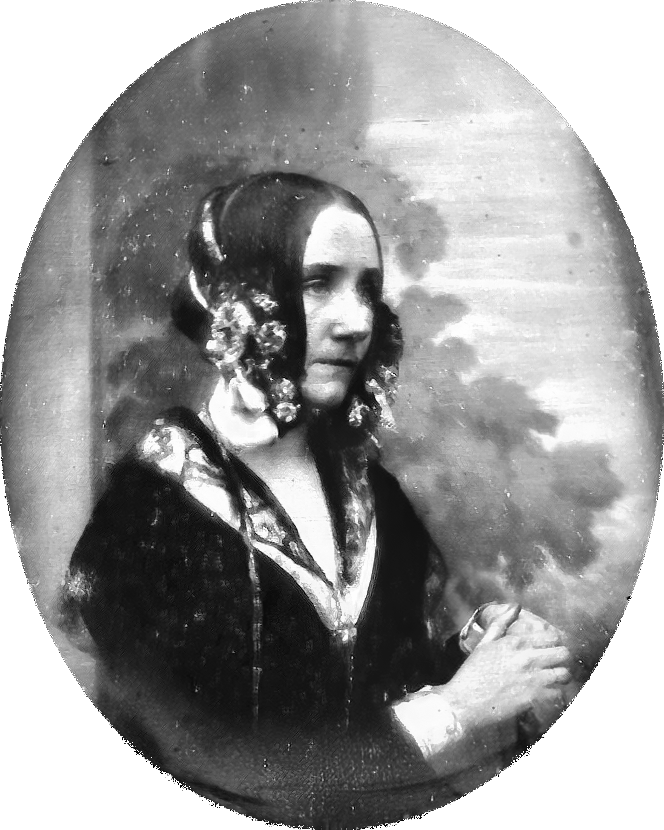
\includegraphics[scale=0.16]{figures/ada.png}
        
        \bigskip
        
        {\scriptsize Augusta Ada King, Countess of Lovelace}
    \end{columns}
    
\end{frame} 

\begin{frame}
    Ada Lovelace's diagram, the first published computer algorithm.
    
    \bigskip
    
    \centerline{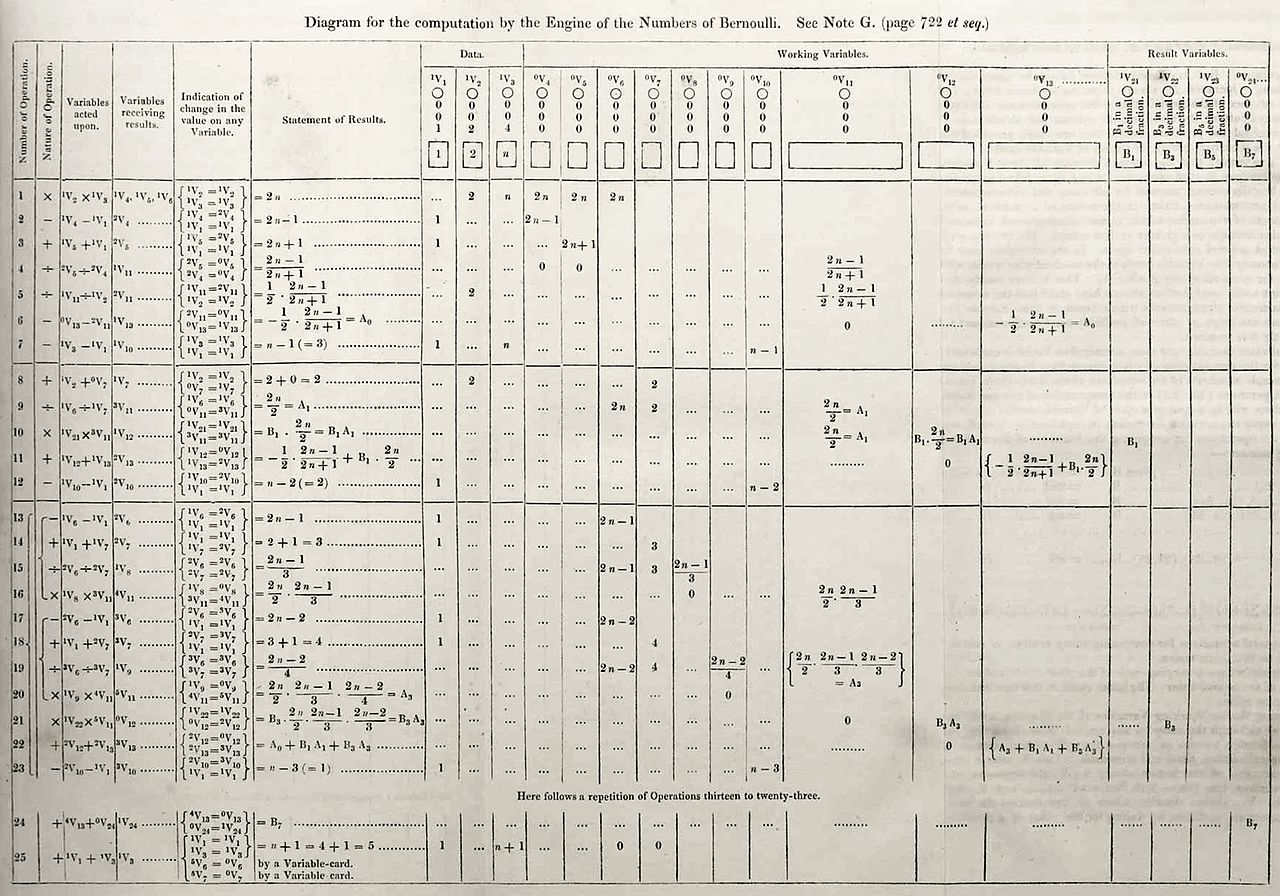
\includegraphics[scale=0.2]{figures/ada_diagram.jpg}}
    
\end{frame}

\section{Algorithms}
\begin{frame}

    \begin{block}{Definition}
        A finite progressive sequence of well-defined (unambiguous) instructions is called an \emph{algorithm}.
    \end{block}

    \bigskip

    \begin{itemize}
        \item Finite
        \item Progressive
        \item Unambiguous
    \end{itemize}

\end{frame}

\begin{frame}

    \begin{alertblock}{Procedures are not algorithms!}
        A simple procedure cannot be safely called an algorithm, since it may be endless. Algorithm must be \emph{finite} both in notation and execution.
    \end{alertblock}    

\end{frame}

\begin{frame}
    Visualizing recipe algorithm

    \centerline{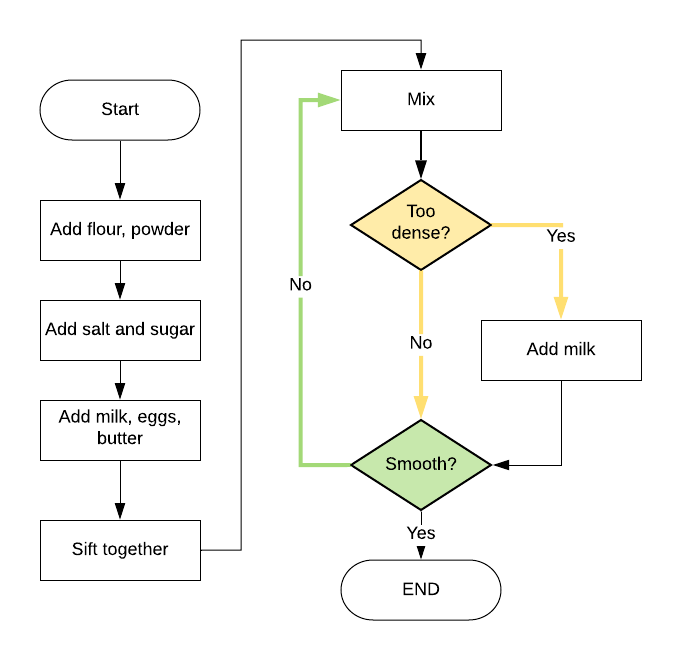
\includegraphics[scale=0.8]{figures/recipe_algo.png}}
    
\end{frame}

\begin{frame}
    Algorithms are represented visually using \emph{flowchart} diagrams.

    \bigskip

    Two key points

    \bigskip

    \begin{itemize}
        \item Branches
        \item Loops
    \end{itemize}
\end{frame}

\begin{frame}

    \begin{block}{Exercise 1}
        Describe the algorithm to resolve the formula
        \begin{align*}
            R = \sum_{n=1}^{10} n
        \end{align*}
    \end{block}    

\end{frame}

\begin{frame}
    \centering
    END
\end{frame}

\end{document}